\chapter{Recuperação de Informação}
\label{cap_2}

Um ativo importante em qualquer organização é a informação. Segundo Kimball e Ross \cite{kimball2002dw} essa informação é mantida sob duas formas: sistemas de banco de dados operacionais e \textit{Data Warehouses}. Em sistemas operacionais geralmente os usuários lidam com o mesmo registro e realizam a mesma tarefa exaustivamente sob uma única informação, permanecendo no domínio das transações; enquanto que em um DW pode-se ver o progresso da organização utilizando dados armazenados continuamente, de forma otimizada para a recuperação de dados. Também, são formuladas perguntas com a finalidade de responder a alguma questão de negócio, como \textit{"quantos pedidos foram recebidos pelo fornecedor X no período de tempo Y?"}, ou \textit{"qual foi o impacto no número de vendas ao mudar o formato de envio de A para B?"}. Para responder questões dessa natureza não é viável lidar com dados de forma individual, mas sim recuperar um conjunto de dados a fim de formular uma resposta.

% \section{\textit{Data Warehouses} e Aplicações OLAP}

De acordo com Inmon \cite{inmon2005building}, DWs são base de todos os Sistemas de Suporte à Decisão (do inglês \textit{Decision Support Systems}, ou DSS). DSS são tecnologias utilizadas para decisões de negócio e solução de problemas, 
e incluem componentes que realizam gerenciamento de banco de dados e que 
permitem uma interação com o usuário de forma a simplificar consultas e geração de relatórios 
\cite{shim2002past}. DWs foram as primeiras ferramentas a surgirem como solução para o 
suporte à decisão de negócio, integrando dados de diferentes bancos de dados operacionais 
\cite{inmon2005building, kimball2002dw}.

De forma geral, um DW é um repositório de dados capaz de fornecer rapidamente 
informações consistentes e cruciais para a tomada de decisão de uma organização, 
de tal forma que essa informação possa ser acessada de maneira intuitiva e legível 
pelo usuário, a fim de combinar diferentes informações entre os dados armazenados 
\cite{kimball2002dw}. Deve também se adaptar a possíveis mudanças, sejam elas mudanças comerciais, mudanças nos dados ou na tecnologia. Inmon \cite{inmon2005building} define um DW como: uma coleção de dados não-volátil, ou seja, que não muda após inserida no \textit{warehouse}; orientado ao assunto principal da organização; integrado e variante no tempo para que seja mantido um histórico a fim de analisar situações passadas. Do ponto de vista estrutural, Wremble e Koncilia \cite{wrembel2007data} definem um DW como uma base de dados homogênea, local e centralizada.

Para analisar os dados de um DW além de implementá-lo é necessário que alguma aplicação leia seu conteúdo e apresente-o de forma gráfica e intuitiva ao analisador. Aplicações OLTP (\textit{On-Line Transactional Processing}) são utilizadas por bancos de dados operacionais e operam transações atômicas e isoladas de forma repetitiva, que correspondem ao dia-a-dia de uma organização \cite{chaudhuri1997overview}. DWs trabalham com suporte à decisão e são intensivos à consultas \textit{ad hoc} complexas, que acessam milhões de registros. Sendo assim, os dados históricos, a taxa de vazão de uma consulta e o tempo de resposta são mais importantes que pequenas transações.

À aplicação aceita por um DW dá-se o nome de OLAP, cujo objetivo, de acordo com Codd; Codd e Salley \cite{codd1998providing}, é identificar tendências, padrões de comportamento e anomalias, bem como relações em dados aparentemente não relacionados. Geralmente as consultas em uma aplicação analítica são longas, levam tempo para executar e estão interessadas 
em atributos específicos. Os resultados dessas análises servem de base para tomada de decisões de negócio. Ainda, o processo de inserção de dados em um ambiente OLAP é um pouco mais complexo que sistemas OLTP por seguir um processo fim-a-fim conhecido 
como ETL (extração, transformação e carga) \cite{vertabelo2017olap}. Portanto, DWs e aplicações OLAP são componentes chave para a construção de um ambiente de análise.

O processo ETL faz parte da arquitetura de um DW. Neste domínio existem diversos componentes que realizam funções específicas a fim de construir um ambiente de \textit{warehouse} desde a obtenção dos dados de fontes externas e sistemas operacionais de bancos de dados, até o acesso a esses dados por meio do DW por alguma consulta analítica definida sob uma aplicação OLAP. Para entender esta arquitetura fim-a-fim, ilustrada na Figura \ref{fig:dw_arq} adaptada de Kimball e Ross \cite{kimball2002dw}, é necessário compreender alguns componentes e conceitos que formam um DW \cite{kimball2002dw}:

\begin{itemize}
    \item \textbf{Sistemas de Fonte Operacional}: possuem detalhes sobre as transações do negócio, correspondendo a ambientes OLTP. Engloba os dados que irão estruturar as informações do DW, portanto se encontram externos ao \textit{warehouse}. Podem ser tanto sistemas de banco de dados ou alguma outra fonte de dados, como um documento no formato XLS, CSV, TXT; e sistemas CRM.
    \item \textbf{\textit{Staging Area}}: compreende tanto uma área de armazenamento temporária quanto um conjunto de processos denominado ETL (\textit{extract-transformation-load}). De forma geral é uma área a qual os usuários não têm acesso, onde os dados são traduzidos para algo que possa ser enviado de maneira compatível ao \textit{warehouse} e não se trabalha diretamente sobre os dados transacionais. Quanto aos processos ETL, a fase de Extração (\textit{Extraction}) consiste na leitura da fonte de dados, transferindo o conteúdo necessário para a \textit{staging area}; após essa extração pode ser necessário realizar uma "limpeza" nos dados; unir dados de diferentes fontes; tratar duplicatas e atribuir chaves do \textit{warehouse}. A isto dá-se o nome de Transformação (\textit{Transformation}). A última fase, fase de Carregamento (\textit{Load}), é responsável por carregar, ou popular, os dados na área de estruturação de dados do DW.
    \item \textbf{Estruturação de Dados}: trata de como os dados serão organizados, armazenados e disponibilizados para consultas de usuários, relatórios e outras aplicações. No que tange à comunidade empresarial, a fase de apresentação de dados \textit{é} o DW em si, pois corresponde ao que pode ser acessado via ferramentas de acesso a dados. A etapa de estruturação é comumente definida como sendo um conjunto de \textit{data marts}. \textit{Data marts} são subconjuntos do total de informações de um DW, cada qual representando os dados de um determinado assunto, departamento, ou processo de negócio. Nesta fase é definida a modelagem conceitual do ambiente de análise do DW.
    \item \textbf{Ferramentas de Acesso aos Dados}: são formas de aplicar uma consulta, dentro de aplicações OLAP, aos dados organizados na fase de estruturação. Pode ser uma consulta \textit{ad hoc} ou algo mais complexo, como consultas aplicadas à mineração de dados.
    
\end{itemize}

\begin{figure*}[htpb]
	\centering
		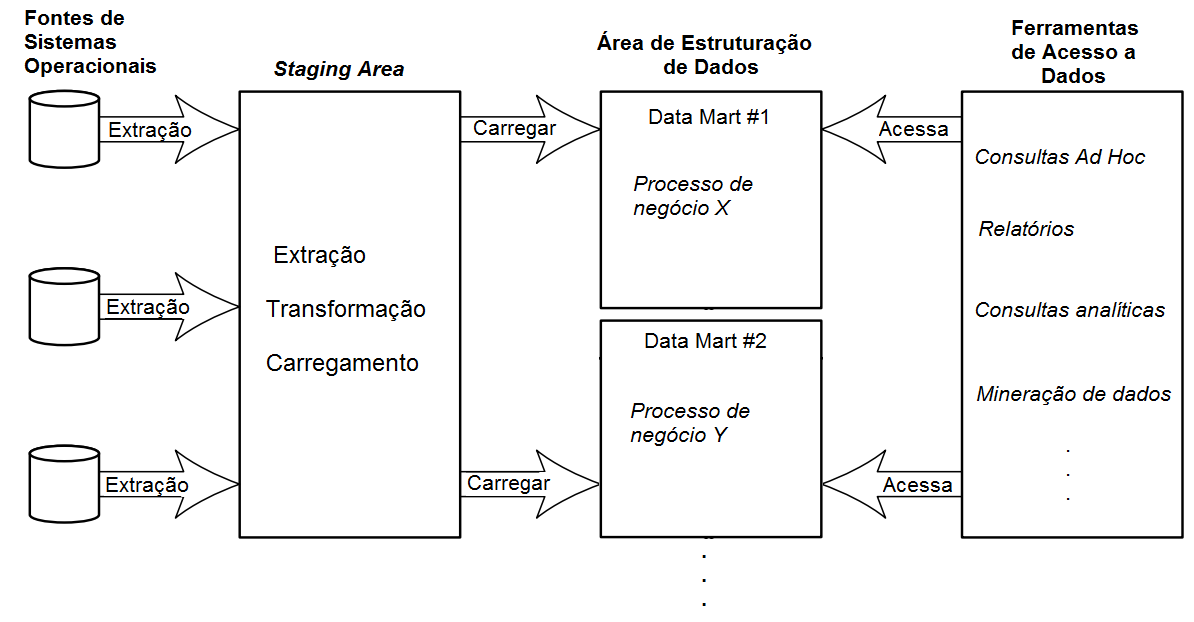
\includegraphics[width=\textwidth]{img/dw_arc}
	\caption{Arquitetura de um \textit{Data Warehouse}.}
	\label{fig:dw_arq}
\end{figure*}

Existe uma discussão acerca da modelagem conceitual da área de apresentação de dados de um ambiente de análise nos DWs \cite{sen2005comparison}. Segundo Sen e Sinha \cite{sen2005comparison} as duas técnicas de modelagem mais utilizadas são a Entidade-Relacional (ER) e a Dimensional. A primeira segue o padrão de modelagem para ambientes OLTP, que traduz a modelagem ER para um esquema relacional em seguida normalizando-o geralmente até a Terceira Forma Normal (3NF) \cite{kimball2002dw}, normalmente utilizadas por bancos relacionais. O modelo Dimensional, ou multidimensional, por sua vez, evita atingir o mesmo nível de normalização da modelagem ER, e faz analogia a um cubo para representação de dados, uma vez que uma informação pode ser vista através de \textit{n} dimensões. 

O modelo dimensional é composto por tabelas denominadas Tabelas Fato e Tabelas Dimensão \cite{kimball2002dw}, e é conhecido comumente como modelo \textit{star join}, ou apenas \textit{star} \cite{sen2005comparison}, pelo seu formato lembrar o de uma estrela. A Tabela Fato é a principal tabela do modelo Dimensional, contemplando atributos responsáveis por determinar as regras e métricas de negócio, ou um fato. Em sua maioria são atributos numéricos, relacionados a quantidade, e aditivos, visto que uma consulta em um DW pode retornar até milhares de tuplas, tornando interessante o conhecimento de informações como o total de um atributo dada alguma questão de negócio. Atributos textuais não são definidos como um fato, na maioria das vezes descrevem algo e devem estar inseridos em Tabelas Dimensão pois há maior chance de estarem relacionados com os atributos dimensão. Outro ponto a se ater é a importância de se evitar incluir dados com zeros que não representam dados úteis, ou representando nada, pois a inclusão de dados sem significado sobrecarregariam o DW sem motivo.

As Tabelas Fato são auxiliadas pelas Tabelas Dimensão no que concerne à descrição textual das questões de negócio. É comum essas tabelas terem de 50 a 100 atributos, ou mais, pois a intenção das dimensões é descrever as regras de negócio. É nestas tabelas que são realizados os filtros de consulta. Por filtros entende-se agrupamentos, padrões e ordenações por exemplo. De forma a exemplificar, se fosse desejado buscar as vendas por nome de fornecedor em um determinado intervalo de data, os atributos "nome de fornecedor" e "data" deveriam estar armazenados em tabelas dimensão. Segundo Kimball \cite{kimball2002dw}, quanto mais bem descritos os atributos dimensão, melhor o DW é, tornando a qualidade do \textit{warehouse} dependente das entidades de dimensão.

Todas as Tabelas Fato tem duas ou mais chaves relacionando-as às Tabelas Dimensão, como mostra o exemplo da Figura \ref{fig:star_dim}, onde a tabela \textit{Vendas} corresponde à uma Tabela Fato e as demais à Tabelas Dimensão. Note que esta figura também faz referência a um modelo \textit{star}.

\begin{figure*}[htpb]
	\centering
		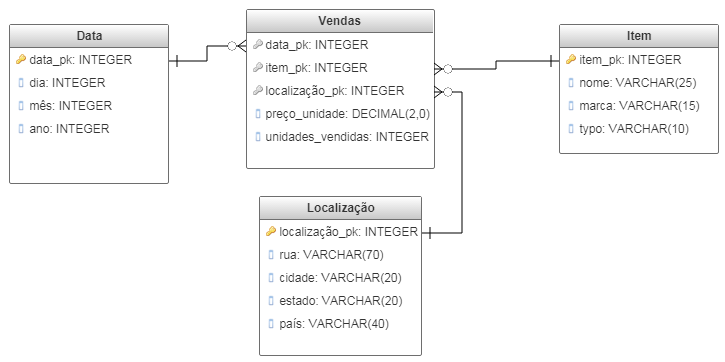
\includegraphics[width=13cm]{img/star_dim}
	\caption{Exemplo de esquema \textit{star} com tabelas Fato e Dimensão}
	\label{fig:star_dim}
\end{figure*}

Mesmo que a modelagem Dimensional não atinja a normalização 3NF, modelos \textit{star} podem ser trabalhados de forma a oferecer suporte à hierarquia de atributos às Tabelas Dimensão, permitindo que estas tenham Tabelas "Subdimensão". A esse refinamento se dá o nome de \textit{snowflake} \cite{navathe2011banco}. Embora tenham uma estrutura mais simplificada, segundo Levene e Loizou \cite{levene2003snowflake} a escolha do uso de esquemas \textit{snowflake} se dá por serem um esquema intuitivo, de fácil entendimento, passíveis à otimização de consultas, e de fácil extensão -- uma vez que pode-se adicionar atributos às tabelas sem interferir em programas já existentes. Uma possível adaptação de um modelo \textit{star} para \textit{snowflake} é como mostrado na Figura \ref{fig:snow}, no qual foi adaptado o modelo da Figura \ref{fig:star_dim}, adicionando a Tabela Subdimensão Cidade. 

\begin{figure*}[htpb]
	\centering
		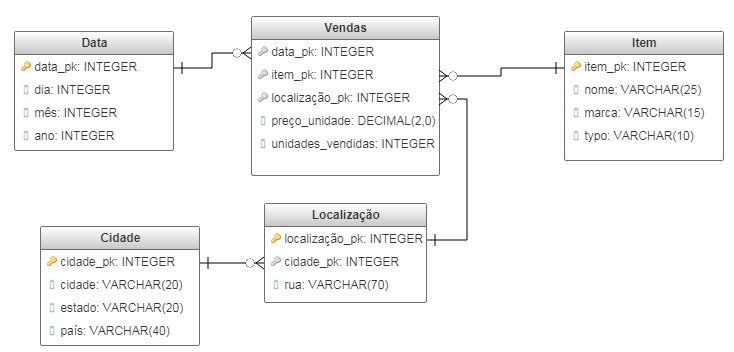
\includegraphics[width=13cm]{img/snow}
	\caption{Exemplo de esquema \textit{snowflake} adaptado da Figura \ref{fig:star_dim}}
	\label{fig:snow}
\end{figure*}

Para que possa ser construído um DW e aplicadas as modelagens acima descritas, 
é necessário alguma ferramenta que possa fazer o gerenciamento dele. 
De acordo com Elmasri e Navathe \cite{navathe2011banco} um banco de dados pode ser gerenciado por sistemas que 
facilitem este processo de gerenciamento no banco de dados. Estes sistemas são conhecidos como Sistemas Gerenciadores de Banco de Dados, ou SGBD.